\documentclass{article}

\usepackage{amsmath}
\usepackage{amsthm}
\usepackage{amssymb}
\usepackage{bbm}
\usepackage{fancyhdr}
\usepackage{cite}
\usepackage{graphicx}
\usepackage{enumitem}
\usepackage{courier}
\usepackage{caption}
\usepackage{listings}
\usepackage{float}
\usepackage{algorithm}
\usepackage{algpseudocode}
\usepackage[pdftex,colorlinks=true, urlcolor = blue]{hyperref}

% \newcommand{d}{\partial}

\oddsidemargin 0in \evensidemargin 0in
\topmargin -0.5in \headheight 0.25in \headsep 0.25in
\textwidth 6.5in \textheight 9in
\parskip 6pt \parindent 0in \footskip 20pt

% set the header up
\fancyhead{}
\fancyhead[L]{Stanford Aeronautics \& Astronautics}
\fancyhead[R]{Fall 2021}

%%%%%%%%%%%%%%%%%%%%%%%%%%
\renewcommand\headrulewidth{0.4pt}
\setlength\headheight{15pt}

\usepackage{xparse}
\NewDocumentCommand{\codeword}{v}{%
\texttt{\textcolor{blue}{#1}}%
}

\usepackage{xcolor}
\setlength{\parindent}{0in}
\twocolumn
\title{AA 228: Decision Making Under Uncertainty \\ Final Project}
\author{Name: Brian Dobkowski and Bianca Jurewicz}
\date{December 3rd, 2021}

\begin{document}

\maketitle
\pagestyle{fancy} 

\section*{Abstract}
This paper considers the problem of an underwater autonomous agent charged with the task of reaching a goal state by traversing an environment with obstacles. To simplify the problem, the 3-dimensional underwater space has been modeled as a 2-dimensional space, allowing only motion along the sea floor. Therefore, a grid-world problem definition can be used to solve the problem.  It is assumed the environment has been previously explored and mapped, which allows the use of offline solution methods to solve the problem. An MDP formulation of the problem is first solved used discrete value iteration, and afterwards a POMDP formulation of the problem is solved using QMDP, FIB, and SARSOP solvers.  All these solutions are compared to the fully-observable MDP solution, and it is described why none of the solutions yield the total expected discounted reward that the MDP solution affords. This paper concludes that the lack of observability has relatively little effect on the partially observable solution given the nature of the problem at hand.

%% There is a reasonable abstract, overview or table of contents present in the paper/presentation. May be written or spoken. %% 

\section*{Introduction}
%% Problem Clearly Stated %%
%% Succinct and clear problem description appropriate for other members of the course.%%
Autonomous cars have given inspiration to a variety of other autonomous vehicles, including autonomous aquatic vehicles.  Underwater robots have a variety of applications such as researching environmental effects, disaster relief for shipwrecks, and deep sea exploration.  As an underwater robot navigates from a starting position to a final position, it must balance efficiency with safety, because it should avoid colliding with obstacles while minimizing the time and energy required to complete a mission. As the robot travels, it may encounter obstacles such as rocks or fish swimming through the sea.  Strong waves may also cause the robot to drift from its intended path and noise from on-board sensors could create uncertainty in the robot's estimate of its own position.
%% Approach Clearly Stated%%
%%Succinct and clear approach description appropriate for other members of the course.%%
%% Appropriateness of Approach %%
%% It is justified why the specific approach in question was chosen for the problem at hand.%%

The problem explored in this paper concerns an autonomous underwater robot charged with the task of reaching a predefined goal state amidst obstacles in the environment.  The approach taken will frame the problem as both a Markov Decision Process (MDP) and a Partially Observable Markov Decision Process (POMDP) to explore different modeling consideration for the problem.  In solving the problem, it will be assumed that the environment has been previously explored by an agent and that an accurate map has been rendered, including boundaries and obstacles.  Therefore, offline methods can be used to solve the MDP and POMDP problems.

\section*{Related Work}

\section*{Modeling}
The 3-dimensional underwater environment can be simplified as a 2-dimensional sea floor environment, treating the robot as an agent that can only move along the plane of the sea floor.  To set up the a POMDP problem, the following seven variables must be defined (only a subset of these is required for the MDP problem) \cite{POMDP Robert}:

\begin{equation}
\langle \mathcal{S}, \mathcal{A}, \mathcal{O}, T, R, O, \mathcal{\gamma} \rangle
\end{equation}

\begin{table}[h]
\centering
\begin{tabular}{c|c}

$\mathcal{S}$ & State Space \\ 
$\mathcal{A}$ & Action Space \\ 
$\mathcal{O}$ & Observation Space \\ 
T & Transition Function\\ 
R & Reward Function \\ 
O & Observation Function \\
$\mathcal{\gamma}$ & Discount Factor \\

\end{tabular}
\end{table}


  The sea floor will be discretized into a 5x5 grid world, resulting in 25 possible states for the position of the robot. A reward of 10 points is assigned to the goal position, which is the farthest state from the initial state. Along its route, the robot will need to navigate around obstacles such as rocks and seaweed. Each obstacle provides a reward value corresponding to its level of damage incurred to the robot. In this example, a rock costs 10 points because a collision would permanently destroy the robot.  Small stagnant fish cost 5 points because they may incur minor damage to the robot and will harm the fish. Lastly, seaweed costs 3 points because it may stick to the robot, too much of which will be overly detrimental to autonomous performance.  The initial state will be $(1, 1)$, while the goal state is $(5, 5)$. The visual representation of the grid world with corresponding reward values is shown in Figure \ref{fig:gridworld}.

\begin{figure}
    \centering
    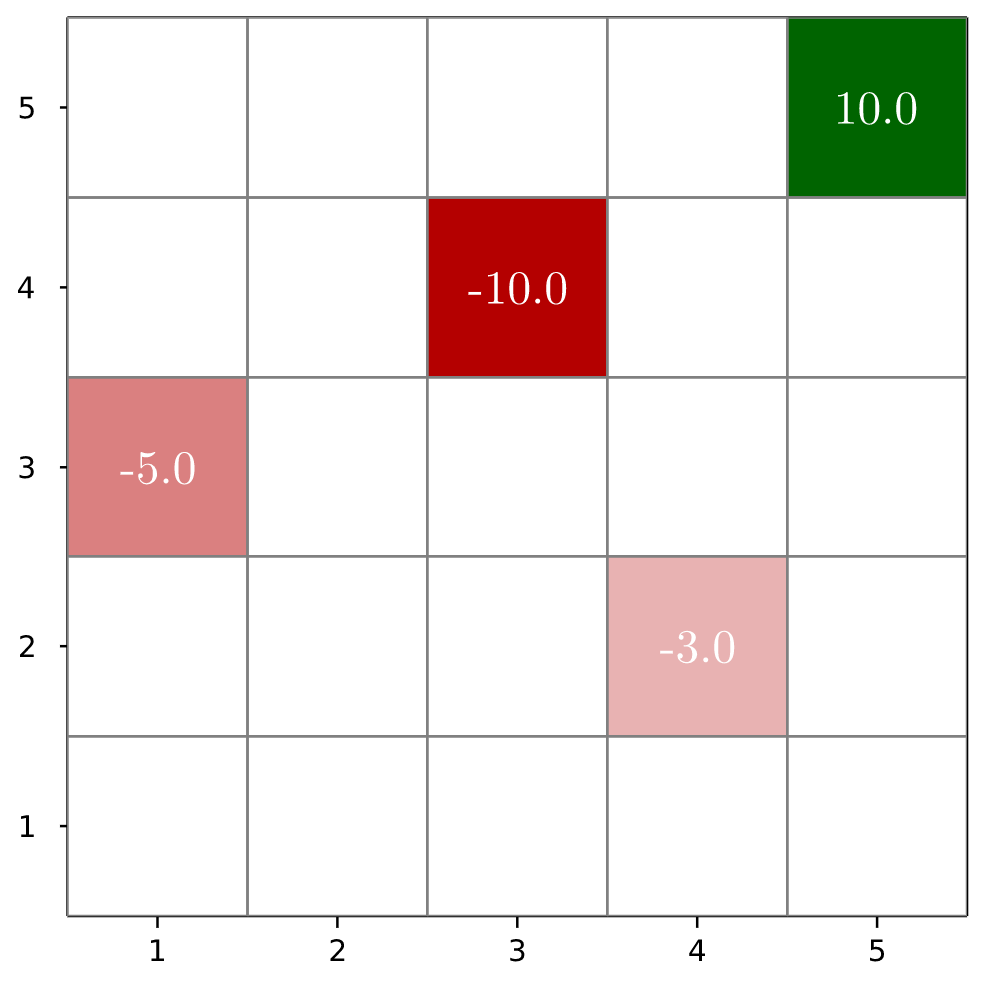
\includegraphics[width=2.5in]{gridworld.png}
    \caption{Grid World representation with reward values displayed.}
    \label{fig:gridworld}
\end{figure}

The robot will be able to take four actions: up, down, left, and right. Due to uncertainties in the environment (e.g. tides, waves, control noise), the robot is unable to deterministically transition from one state to any neighboring state. It was desired to tie this transition function to a robot's dynamical equations, but for simplicity of analysis, this paper presents a probabilistic transition model. With a probability of 80$\%$, the robot transitions to the desired state.  The remaining 20$\%$ probability is evenly split between neighboring states that are within the bounds of the problem.
  
This paper will also compare observation models and evaluate how the observation model affects the policy computed.  This paper will analyze 4 observation models corresponding to a 70$\%$, 80$\%$, 90$\%$, and 100$\%$ probability that the observed state is the robot's true state.  Similar to the transition function, the remaining likelihood (if any) is evenly distributed between the adjacent states provided they are within the bounds of the problem. Finally, this example uses a discount factor of 0.9.

This paper will first present the problem as an MDP assuming full observability of the robot's current state. This implementation will serve as a baseline against which to compare the partially observable case, in which the quality of observation will be degraded for analysis. Though various methods can be used to solve for an optimal policy for both MDPs and POMDPs, offline methods were examined in this paper.  These methods were used because the problem posed assumes a mapped sea environment, a known beginning state, and a known end state. The initial belief is deterministically set to the initial state. This approach acknowledges that alternative online methods would need to be investigated if an autonomous robot in an unknown environment was being designed for, and thus would need some exploration component.

\section*{Evaluation Metrics}
To evaluate the efficacy of the optimal policy solved for in both the MDP and POMDP formulations of this problem, a Monte Carlo simulation technique will be used. For each solution, 15,000 independent simulations were run from the initial state.  For the MDP optimal policy, each state is mapped to only one action, so the actions are chosen according to what state the robot is currently in. For the POMDP set of alpha vectors, a greedy action selector was implemented, which is given by the below equation. This action was selector was chosen out of simplicity rather than use the one-step lookahead function.

\begin{equation}\label{greedyaction}
    a = \underset{a}{\arg\max}\,\alpha^Tb
\end{equation}

To ensure consistent performance, a simulator was built from scratch to evaluate these policies, rather than use the pre-programmed POMDP simulators that have implementations specific to each solver. For each solution, the sum of discounted rewards was collected as in the equation below.

\begin{equation}\label{discountreward}
    R_{sim} = R_{s0} + \gamma R_{s1} + \gamma^2 R_{s_3} + \cdots
\end{equation}

When the robot reaches a terminal state (i.e. any obstacle or the goal), the simulation for that specific trajectory ends. When all simulations have been completed, a solution's policy is judged based on its mean discounted reward over all the simulation samples.


\section*{MDP Formulation and Solution}
A Markov Decision Process (MDP) will serve as the baseline case.  Under an MDP, there is no state uncertainty.  The optimal policy for an MDP can be calculated through Value Iteration using Equation \ref{val_it}:

\begin{equation}\label{val_it}
    \pi^*(s) = \underset{a}{\arg\max} \left( R(s,a) + \gamma \sum_{s'}T(s' \mid s,a)U^*(s')\right)
\end{equation}

% \begin{align}\label{val_it}
%     U^*(s) &= \max_{a} \left( R(s,a) \\
%     &+ \gamma \sum_{s'}T(s' \mid s,a)U^*(s')\right)
% \end{align}

By implementing Equation \ref{val_it} on the underwater robot grid world, the optimal policy defines the best action to take in each state of the grid world.  Figure \ref{fig:optimal} below visualizes the optimal policy for the robot.

\begin{figure}[h]
    \centering
    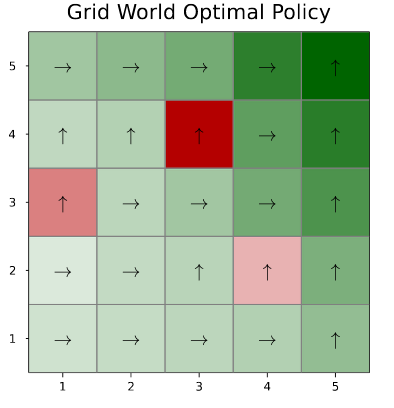
\includegraphics[width=2.6in]{optimal.png}
    \caption{Optimal Policy determined by value iteration, including a soft visualization of the utility of being in each individual state.}
    \label{fig:optimal}
\end{figure}

Simulating the MDP through 15,000 iterations resulted in an average discounted reward of 1.835.  This is the discounted reward associated with the true optimal policy, so the POMDP methods are expected to return rewards less than or equal to this value.  Two policies can be compared by evaluating which one returns an average discounted reward that is closer to the reward associated with the optimal policy, 1.835.

\section*{POMDP Solution Methods}
Three different solvers were used to solve for optimal policies with the POMDP-version of the problem.  All solvers define a policy as a set of alpha vectors over the belief space, though the number of these alpha vectors varies with each method. To extract the optimal action given a final set of alpha vectors and a belief, a greedy action selector as in Equation \ref{greedyaction}.

\subsection*{QMDP}

The QMDP offline planning method computes a set of alpha vectors to define a policy.  It computes one alpha vector for each action through value iteration \cite[21.1]{228 Book}.  The equation to compute the alpha vector is defined by Equation \ref{qmdp_alph}:

\begin{equation}\label{qmdp_alph}
    \alpha_{a}^{(k+1)}(s) = R(s,a) + \gamma \sum_{s'}T(s' \mid s,a)\max_{a'}\alpha_{a'}^{(k)}(s')
\end{equation}

Note that QMDP assumes full observability in the system after taking the first step. Therefore, the different observation models should have no effect on the solution. It was verified that QMDP converges to the same set of alpha vectors regardless of the observation model used. The difference in performance is manifested in the simulations - with a higher confidence observation, the robot is able to localize itself better which improves its belief when using the discrete updater. This improves the performance of the greedy action selector. Due to its assumptions, QMDP provides an upper bound on the optimal value function.

Table \ref{tab:qmdp} contains the average discounted reward generated from 15,000 simulations of the QMDP method for various observation distributions.

\begin{table}[h]
\centering
\caption{QMDP Simulation Results}
\label{tab:qmdp}
\begin{tabular}{|c|c|}
\hline
O & Average Discounted Reward  \\ \hline
0.7 & 1.68 \\ \hline
0.8 & 1.72 \\ \hline
0.9 & 1.81 \\ \hline
1.0 & 1.832 \\ \hline
\end{tabular}
\end{table}

\subsection*{FIB}

The Fast Informed Bound (FIB) offline planning method is another method that computes alpha vectors to define a policy \cite[21.2]{228 Book}.  FIB computes one alpha vector for each action using Equation \ref{fib_alph}:

\begin{multline}\label{fib_alph}
    \alpha_{a}^{(k+1)}(s) = R(s,a) + \\ \gamma\sum_{o}\max_{a'}\sum_{s'}O(o \mid a,s')T(s' \mid s,a)\alpha_{a'}^{(k)}(s')
    \end{multline}

Note that FIB takes into account the observation model to some extent, which suggests it will provide a tighter upper bound than QMDP.

Table \ref{tab:fib} contains the average discounted reward generated from 15,000 simulations of the FIB method for various observation distributions.

\begin{table}[h]
\centering
\caption{FIB Simulation Results}
\label{tab:fib}
\begin{tabular}{|c|c|}
\hline
O & Average Discounted Reward  \\ \hline
0.7 & 1.706 \\ \hline
0.8 & 1.748 \\ \hline
0.9 & 1.770 \\ \hline
1.0 & 1.835 \\ \hline
\end{tabular}
\end{table}

\subsection*{SARSOP}

Successive Approximations of the Reachable Space under Optimal Policies (SARSOP) is a Point-Based POMDP algorithm.  Point-based algorithms sample from the belief space instead of iterating over the entire belief space.  With SARSOP, the sampling is taken from the reachable belief space of the optimal policy. The optimal policy is unknown, so a lower bound is kept on the optimal policy as an approximation \cite{SARSOP}.  Figure \ref{fig:sarsop tree} visually depicts the sampled points from the reachable belief space as a tree, $T_{\mathcal{R}}$, where each node in the tree is a sampled point \cite{SARSOP}.  Algorithm \ref{alg:sarsop} defines the method as follows \cite{SARSOP}:

\begin{figure}[h]
    \centering
    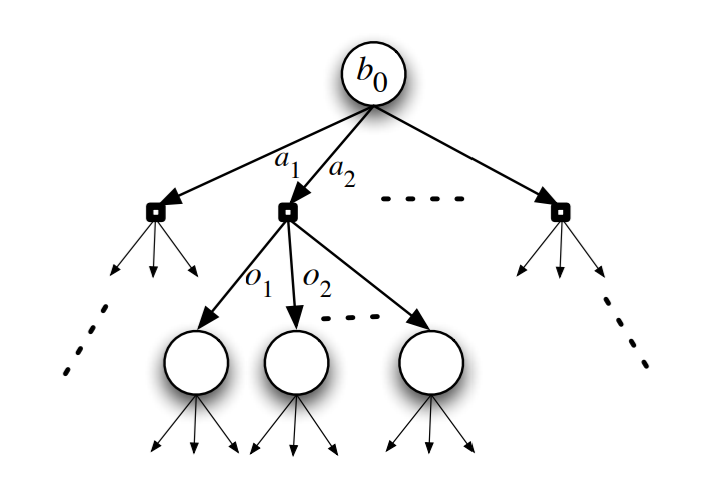
\includegraphics[width=2.5in]{sarsop.png}
    \caption{Belief tree $T_{\mathcal{R}}$ rooted at $b_{0}$.}
    \label{fig:sarsop tree}
\end{figure}

\begin{algorithm}
\caption{Psuedocode for SARSOP Method}\label{alg:sarsop}

Initialize the set $\Gamma$ of $\alpha$-vectors, representing the lower bound $\underline{U}$ on the optimal value function $U^*$.

Insert the initial belief point $b_{o}$ as the root of the tree $T_{\mathcal{R}}$
\begin{algorithmic}
\Repeat
    \State \Call{sample}{$T_{\mathcal{R}}$,$\Gamma$}
    \State Choose a subset of nodes from $T_{\mathcal{R}}$.
    \State For each chosen node $b$, \Call{backup}{$T_{\mathcal{R}}$,$\Gamma$,$b$}
    \State \Call{prune}{$T_{\mathcal{R}}$,$\Gamma$}
\Until termination conditions are satisfied.

\textbf{return} $\Gamma$
\end{algorithmic}
\end{algorithm}

Table \ref{tab:sarsop} contains the average discounted reward generated from 15,000 simulations of the SARSOP method for the various observation models.

\begin{table}[h]
\centering
\caption{SARSOP Simulation Results}
\label{tab:sarsop}
\begin{tabular}{|c|c|}
\hline
O & Average Discounted Reward  \\ \hline
0.7 & 1.70 \\ \hline
0.8 & 1.73 \\ \hline
0.9 & 1.78 \\ \hline
1.0 & 1.826 \\ \hline
\end{tabular}
\end{table}

%% Analysis and Results %%
%% The approach described was quantitatively analyzed according to a set of clearly described metrics, and the results of this analysis presented as figures/tables/graphs/etc. %%

%% Clarity of Drawings, Graphs, Tables %%
%% The drawings, graphs and tables included support the points that are made in the paper/presentation. Complex concepts that require diagrammatic or visual presentation are appropriately presented. %%

Figure \ref{fig:gengraph} depicts a conditional plan for a simplified $3x3$ grid world as an example. The initial state is (1, 1), with an initial belief of 100$\%$ in (1, 1). One can see that there is a 70$\%$ chance the observed state is the next state in the transition, and that the remaining 30$\%$ is split between the two adjacent states that are in bounds (up and right). The state/belief indices go up to 18 in this example, only because there are two representations of the 9 states of the system (9 grid states with terminal set to false, and the same 9 grid states with terminal set to true). If a state is terminal the simulation exits and the process is complete.

\begin{figure}[H]
    \centering
    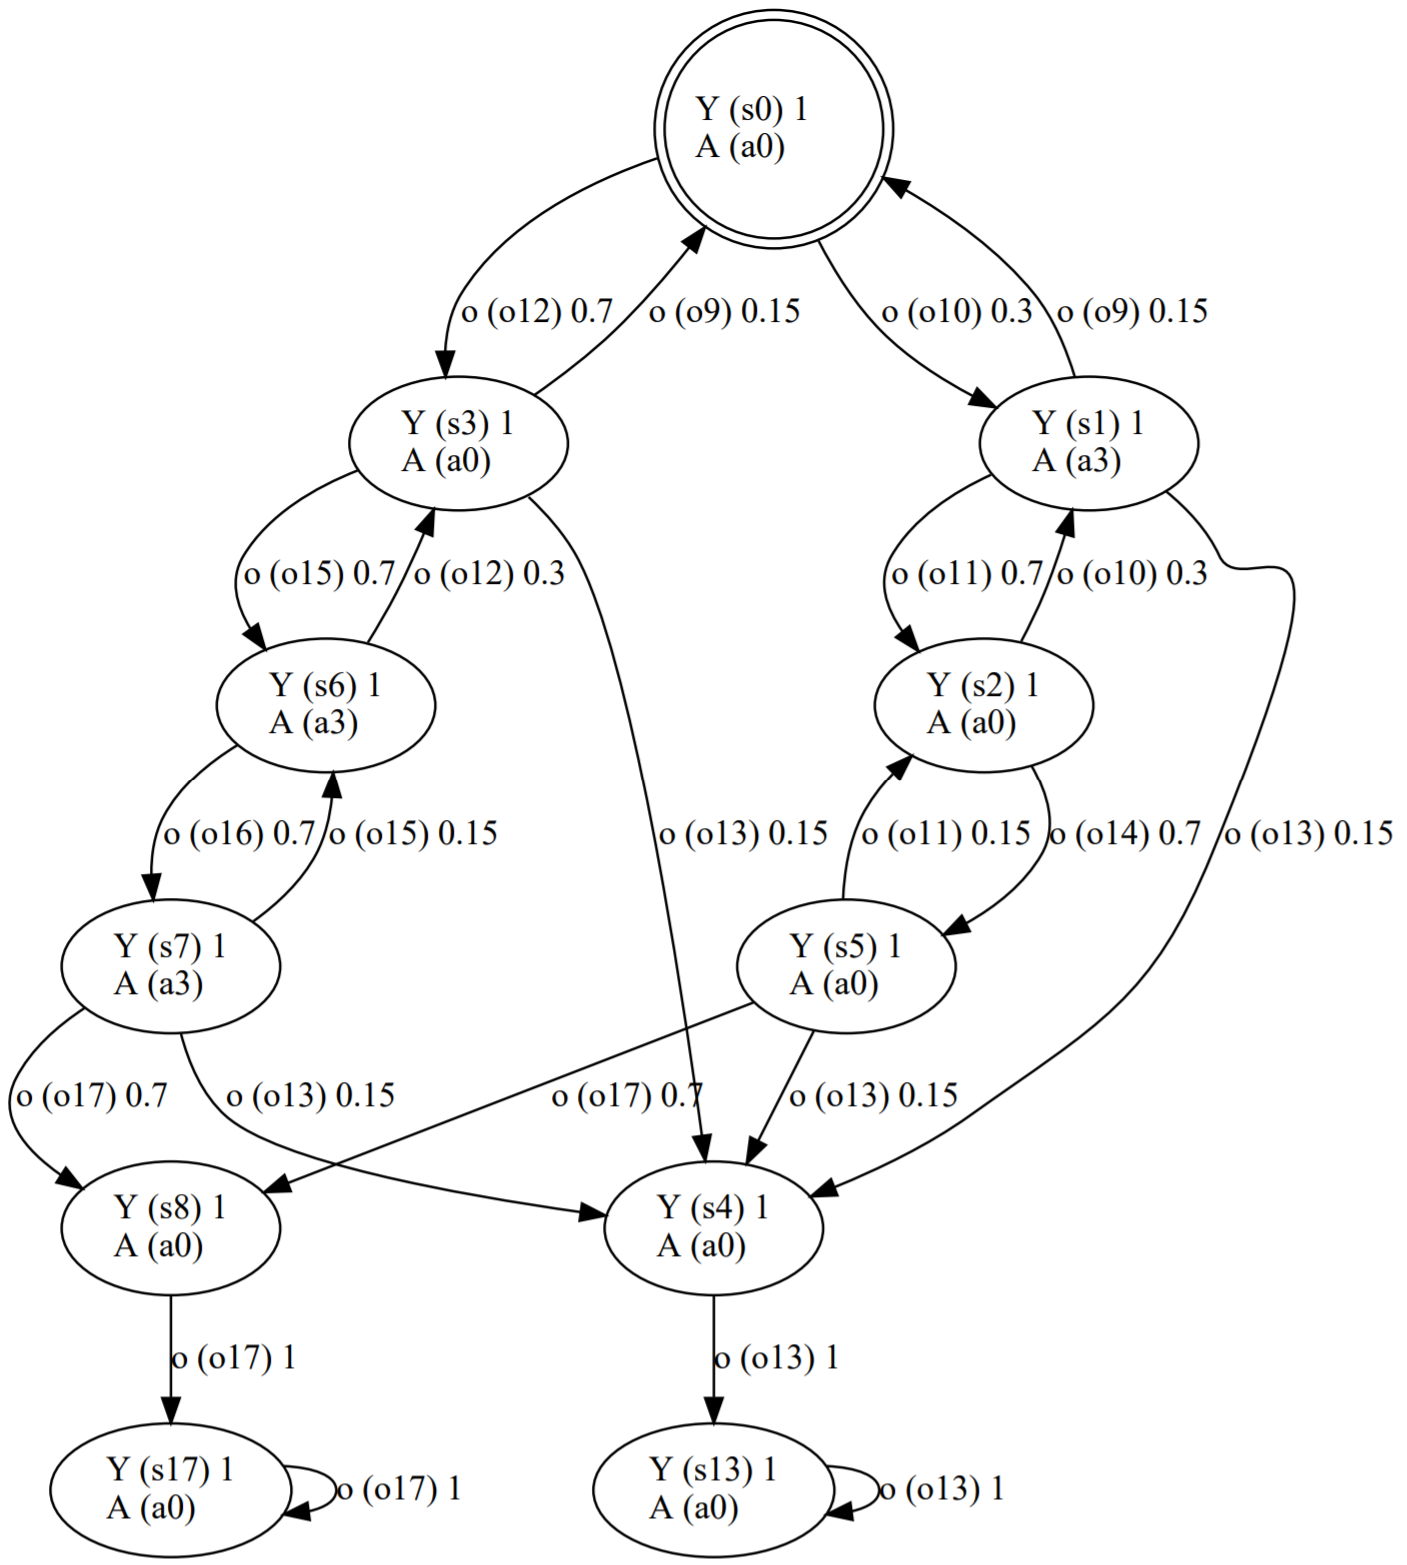
\includegraphics[width=3in]{gengraph.png}
    \caption{Graph Generated by SARSOP Policy for 3x3 world.}
    \label{fig:gengraph}
\end{figure}



\section*{Analysis and Results}


Each offline method used to solve the POMDP successfully converged to a set of alpha vectors the underwater robot to use when navigating the grid world. Table \ref{tab:all} compares the average discounted reward generated from 15,000 simulations of each offline method (QMDP, SARSOP, and FIB) for various observation distributions.

\begin{table}[H]
\centering
\caption{Simulation Results for Various Solvers}
\label{tab:all}
\begin{tabular}{|c|c|c|c|}
\hline
O & QMDP & SARSOP & FIB \\ \hline
0.7 & 1.68 & 1.70 & 1.706 \\ \hline
0.8 & 1.72 & 1.73 & 1.748 \\ \hline
0.9 & 1.81 & 1.78 & 1.770 \\ \hline
1.0 & 1.832 & 1.826 & 1.835 \\ \hline
\end{tabular}
\end{table}

As the observation probability increased, the expected reward increased for each POMDP solver.  This makes sense because as observability improves, the robot has higher confidence in its belief state and can better choose actions that maximize utility from the current state of operation. At full observability, each POMDP method produces the same (or very nearly the same) expected reward as the baseline MDP case, which was expected. This signifies that for the problem at hand, each solution method provides comparable results to value iteration in the fully observable case. Overall variation in performance with the different observation models is quite low, however (only 8.5$\%$ of maximum expected reward variation among all observability trials). More variation was expected here, but this analysis suggests that the greedy action selector may not be as discerning with the different observation models. The team assumes a one-step lookahead action selector would improve this variability among solutions. It is also interesting to note that FIB's solutions do not provide tighter bounds than QMDP's solutions, as is expected given the fact that FIB considers the observation model whereas QMDP does not. This may highlight the simulation method of analysis is susceptible to probabilistic randomness, or that not enough simulations were run. Figure \ref{fig:fib_policy} visualizes a trajectory using a policy generated by FIB, which coincidentially matches the optimal policy for the baseline MDP case in Figure \ref{fig:optimal} when the agent begins in the state (1, 1)..

\begin{figure}
    \centering
    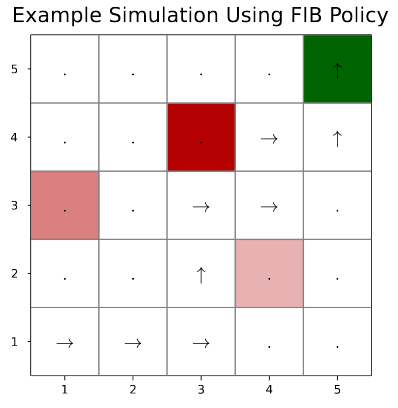
\includegraphics[width=2.5in]{fibpolicy.png}
    \caption{Visualization of the actions chosen in a particular (successful) simulation using the FIB-solved set of alpha vectors.}
    \label{fig:fib_policy}
\end{figure}

It is also important to keep in mind that the three methods have different computation complexities associated with them.  QMDP has a computational complexity of $O(\mid\mathcal{A}\mid ^2\mid\mathcal{S}\mid^2)$, FIB has a complexity of $O(\mid\mathcal{A}\mid ^2\mid\mathcal{S}\mid ^2\mid\mathcal{O}\mid)$, and the complexity of SARSOP depends on the number of samples extracted.  Complexity may be a factor in deciding which method to use for a specific application.

\section*{Conclusion}
A POMDP is an appropriate method to represent a robot autonomously driving towards a goal position with uncertainty in its state transitions and observations.  The QMDP, FIB, and SARSOP methods all converge to the optimal policy and return a larger expected reward as the amount of observability increases, which indicates the solvers are operating correctly and converging to satisfactory policies.  Though the expected trends exist in regards to different observabilities (greater observability is correlated with more expected reward), the benefit of improved observability was not all that stark. This is attributed mostly to the action selection function rather than the solution methods themselves.  This finding may also be an artifact of the particular problem that was framed.

\section*{Future Work}

In future iterations of this project, the greedy action selector should be replaced with a one-step lookahead action selector to provide more variability (and hopefully more optimistic solutions) in regards to different observation models. Also, it would be good to tie the transition function to the robot's actual dynamics, rather than providing an arbitrary probability function. Similarly, the observation model would be a result of studying the robot's actual on-board sensing capabilities, rather than creating an arbitrary function for analysis.

Although the offline methods can all be run to convergence, in practice, online methods may better suit a particular application.  The offline methods rely on having a known map and therefore limit the scope of applications. An online method such as Monte Carlo Tree Search would be an appropriate online method alternative.

\section*{Acknowledgements}
% Cite Robert's program and tiger pomdp
% POMDPs.jl Library
% SARSOP library
We used the \verb!POMDPs.jl! library as a reference for constructing the MDP grid world \cite{POMDPs.jl}.  Then, we adapted the observation function from the \verb!Tiger.ipynb! example to our grid world POMDP \cite{tiger}.  We also used Robert Moss's notebook, ``Partially Observable MDPs'' as a reference in constructing our POMDP \cite{POMDP Robert}.

Both partners brainstormed the problem, modeled it in Julia together, and decided on solution methods to use. Brian worked on other programming tasks, such as creating a new simulator for the project, creating the observation model, and creating visualizations for results.  Bianca worked on code debugging, formulation of project goals, and took the lead on the project write up.  Both members analyzed the results and tied them back to class concepts.

%\onecolumn
\begin{thebibliography}{}
\bibitem{POMDP Robert} Robert Moss, ``Partially Observable MDPs'', https://htmlview.glitch.me/?https://github.com/
JuliaAcademy/Decision-Making-Under-Uncertainty/blob/master/html/2-POMDPs.jl.html
\bibitem{228 Book} Mykel J. Kochenderfer, Tim A. Wheeler, and Kyle H. Wray, ``Algorithms for Decision Making'', MIT Press, 2022.
\bibitem{SARSOP} Kurniawati, Hanna, et al. SARSOP: Efficient Point-Based POMDP Planning by Approximating Optimally Reachable Belief Spaces, https://www.roboticsproceedings.org/rss04/p9.pdf. Robotics: Science and Systems, 2008. Accessed 1 Dec. 2021. 
\bibitem{POMDPs.jl} Github, POMDPs.jl Package, https://github.com/JuliaPOMDP/POMDPs.jl
\bibitem{tiger} Github, ``Tiger Tutorial: Solving POMDPs'', https://github.com/JuliaPOMDP/
POMDPExamples.jl/blob/
cdc8339db795b7d57b80550b52e1d708a584bb9c/
legacy/Tiger.ipynb.
\end{thebibliography}
\end{document}
